\documentclass[12pt]{article}

% Language setting
\usepackage[utf8]{inputenc}
\usepackage[bulgarian]{babel}

% --------------------- Packages  --------------------
% Use biblatex
\usepackage{biblatex}
\addbibresource{bibliography.bib}
% Table thickness
\usepackage{ctable}
% Equations: SI units
\usepackage{siunitx}
% Approximately equal
\usepackage{amssymb}
% degrees symbol
\usepackage{gensymb}
% warning box
\usepackage{pifont,mdframed}
% Multiline math
\usepackage{amsmath}

\newenvironment{warning}
  {\par\begin{mdframed}[linewidth=2pt, linecolor=white]%
    \begin{list}{}{\leftmargin=1cm
                   \labelwidth=\leftmargin}\item[\Large\ding{43}]}
  {\end{list}\end{mdframed}\par}

% --------------------- Title  --------------------
\addbibresource{bibliography.bib}

\begin{document}

% Anfang der Titelseite________________________________________________________________________________
\begin{titlepage}
	\flushleft
	{\scshape\Large Протокол VIII \hspace{2cm} Молекулна физика\par}
	\vspace{4cm}
	{\huge\bfseries Измерване на специфична топлина на изпарение на течност и специфична топлина на топене на лед\par}
	\vspace{1cm}
	{\LARGE\bfseries Лабораторно упражнение №3.14\par}
	\vspace{4cm}
    {\LARGE\bfseries Виолета Кабаджова, \par}
    {\large\bfseries ККТФ, фак. номер: 3PH0600026\par}
	\vspace{1cm}
	
	{\large Физически Факултет, 
	
	Софийски Университет "Св. Климент Охридски"
	
	02 юни 2023 г.\par}
	
\end{titlepage}

\section{Теоритична част}\label{sec:theoretical-part}
За изолирана термодинамична система, можем да запишем така нареченото уравнение на топлинния баланс (ур. \ref{eq:thermal-equilibrium-1}) - отдадената от по-топлите тела количество топлина $Q_j$ е равно на приетото количество $Q_i$ от по-студените тела. Тъй като за изохорен процес може да се запише уравнение \ref{eq:q-du}, където $c_V$ - специфичен топлинен капацитет на идеален газ, $M$ - масата му, $\Delta T = T_{KP} - T_H$ - разликата между крайната и началната температура, и за твърди тела и течности поради малка промяна на обемите им с температурата, може да се приеме $c_V \equiv c$ и ур. \ref{eq:thermal-equilibrium-1} да се запише във вида \ref{eq:thermal-equilibrium-2}.

\begin{equation}\label{eq:thermal-equilibrium-1}
    \Sigma_{j=1}^mQ_j = \Sigma_{i=1}^mQ_i
\end{equation}

\begin{equation}\label{eq:q-du}
    Q = \Delta U = c_V M \Delta T = c_V M (T_{KP} - T_H) 
\end{equation}

\begin{equation}\label{eq:thermal-equilibrium-2}
    \Sigma_{j=1}^mc_jM_j(T_j - \theta) = \Sigma_{i=1}^mc_iM_i(\theta - T_i)
\end{equation}

При протичане на фазов преход в системата, то обмененото количество топлина за неговото осъществяване също трябва да бъде взето в предвид в уравнението на топлинния баланс, като за фазов преход изпарение (кондензация) то е $Q = \lambda M$, а за фазов преход топене (втвърдяване, кристализация) е $Q = rM$, където $\lambda$, $r$ са съответно специфични топлини на изпарение и топене, [$\lambda$] = J/kg, [$r$] = J/kg.  

При постъпването на водна пара в топлинно изолиран от околната среда съд с вода, най-напред парата се втечнява (настъпва фазов преход от I род), при което се отделя количество топлина $Q_1 = \lambda M_{steam}$, където $M_{steam}$ е масата на парите. След това втечнената пара се охлажда до крайна до този момент в съда температура $T_{KP}$. В следствие на това в съда се отделя количество топлина $Q_2 = c_B M_{steam}(T_K - T_{KP})$. Получените количества топлина $Q_1$ и $Q_2$ нагряват съда от начална температура $T_H$ до крайна температура $T_{KP}$. Съответните количества топлина, погълнати от водата и съда са $Q_3 = C_C(T_{KP} - T_H$ и $Q_4 = c_BM_B(T_{KP} - T_H)$. Тогава уравнението на топлинния баланс придобива вида $Q_1 + Q_2 = Q_3 + Q_4$ или вида на уравнение \ref{eq:thermal-equilibrium-3} и оттам изразяваме $\lamda$ във вида на уравнение \ref{eq:latent-vaporization-heat-water}, където $M_{steam}$ е масата на парите в изследвания съд, $c_B$, $M_B$ са специфичния топлинен капацитет и масата на водата, $T_H$, $T_{KP}$, $T_K$ са съответно начална, крайна температура и температура на кипене на водата, $C_C$ - топлинен капацитет на дюаровия съд.

\begin{equation}\label{eq:thermal-equilibrium-3}
    \lamda M_{steam} + c_BM_{steam}(T_K - T_{KP}) = C_C(T_{KP} - T_H) + c_BM_B(T_{KP} - T_H)
\end{equation}

\begin{equation}\label{eq:latent-vaporization-heat-water}
    \lambda = \frac{1}{M_{steam}}
    \left[(T_H - T_{KP})(C_C + c_BM_B) - c_BM_B(T_{K} - T_{KP})\right]
\end{equation}


По подобни на горните разсъждения може да се достигне и до формулата за намиране на специфичен топлина на топене (ур. \ref{eq:latent-melting-heat-ice}) при слагането на кубчета лед в топлинно изолиран съд. Във формула \ref{eq:latent-melting-heat-ice} $M_{ice}$ е масата на леда, $c_B$, $M_B$ са специфичния топлинен капацитет и масата на водата, $T_H$, $T_{KP}$, $T_T$ са съответно начална, крайна температура и температура на топене на леда, $C_C$ - топлинен капацитет на дюаровия съд.  

\begin{equation}\label{eq:latent-melting-heat-ice}
    r = \frac{1}{M_{ice}}\left[(T_H - T_{KP})(C_C + c_BM_B) - c_BM_{ice}(T_{KP} - T_T)\right]
\end{equation}

\section{Експериментална част}

\subsection{Експериментална установка}
% \begin{figure}
%     \centering
%     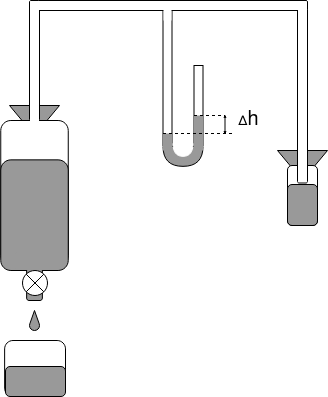
\includegraphics[width=0.5\textwidth]{images/surface-tension-setup.png}
%     \caption{\label{fig:setup}Схема на опитна постановка}
%     \label{fig:setup}
% \end{figure}

В таблица \ref{tbl:constants} са дадени стойностите на константите, използвани по-долу в пресмятанията. 

\subsection{Задача: Измерване на специфична топлина $r$ на топене на лед}
Слагаме няколко кубчета лед във вода с начална температура $T_H$ = 20.9 \degree C и маса $M_B$ = 150 ml = 0.15 kg и разбъркваме добре до пълното разтопяване на леда при температура $T_K$ = 7.6 \degree C. Масата на леда определяме от разликата на крайната маса (с разтопения лед) и началната (със сложения във водата неразтопен лед): $M_{ice} = 0.1 \cdot 10^{-3}$ kg. Смятаме специфичната топлина на топене по формула \ref{eq:latent-melting-heat-ice}.

Температурата на топене на леда $T_T$ се взима таблично за съответното налягане. В нашия случай (стандартни условия с налягане $p = 101.3$ kPa), тя е $T_T = 0$ \degree C. Прилагайки формула \ref{eq:latent-melting-heat-ice}, получаваме r = $(282.9 \pm 0.8) \cdot 10^3$ J/kg. Грешката пресмятаме по формула \ref{eq:abs-err-r}.

\begin{equation}\label{eq:abs-err-r}
    \Delta r = r\left[\frac{\Delta T_H}{T_H} + \frac{\Delta T_{KP}}{T_{KP}} + \frac{\Delta T_K}{T_K} + \frac{\Delta M_B}{M_V} + \frac{\Delta M_{ice}}{M_{ice}} + \frac{\Delta c_{B}}{c_{B}} + \frac{\Delta C_C}{C_C}\right]
\end{equation}

\subsection{Задача: Определяне на специфична топлина $\lambda$ на изпарение на водата}
\begin{figure}
    \centering
    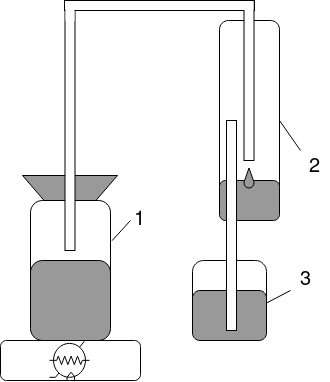
\includegraphics[width=0.3\textwidth]{images/setup-water-vaporization.png}
    \caption{\label{fig:setup-vaporization}Схема на опитна постановка при измерване на специфичната топлина на изпарение на вода: 1 - парогенератор (вода в съд върху нагревател), 2 - дефлегматор, 3 - течност, нагряваща се от парите в дефлегматора.}
\end{figure}

В дюаровия съд отново се налива дестилирана вода, като се записва нейната начална температура $T_H = 19.8 \degree $ C след като е достигнала термично равновесие със съда, в който е поставена. Включваме парогенератора, който е свързан към дюаровия съд през дефлегматор (фиг. \ref{fig:setup-vaporization}). Водата от съд 1 започва да се изпарява, парите достигат до дефлегматора и оттам достигат до съд 3 с изследваната течност, която започва да се нагрява от парите, които достигат до близо сантиметър от дъното на съда. Когато температурата на водата в съд 3 достигне $T_{KP} = 53.2 \degree$ C, изключваме парогенератора и прекъсваме връзката на изследвания съд с останалата част от системата. Измерваме масата на парите като разлика от масата на водата преди и след експеримента и заместваме стойностите във формула \ref{eq:latent-vaporization-heat-water}, изчислявайки специфичната топлина на изпарение на водата $\lamda = (2671 \pm 35) \cdot 10^3$ J/kg. Грешката пресмятаме по формула \ref{eq:abs-err-lambda}.

\begin{equation}\label{eq:abs-err-lambda}
    \Delta \lambda = \lambda\left[\frac{\Delta T_H}{T_H} + \frac{\Delta T_{KP}}{T_{KP}} + \frac{\Delta T_K}{T_K} + \frac{\Delta M_B}{M_V} + \frac{\Delta M_{steam}}{M_{steam}} + \frac{\Delta c_{B}}{c_{B}} + \frac{\Delta C_C}{C_C}\right]
\end{equation}

\begin{table}[h]
\begin{center}
\begin{tabular}{|l|l|l|} \hline
    Величина & Стойност & Мерна единица \\ \hline
    Специфичен топлинен капацитет $c_B$ & & \\ 
    на водата при температура T = 20 \degree C и & 4.1816 \cdot 10^3 & J/(kg.K) \\ 
    налягане p = 101.3 kPa & & \\ \hline
    Температура на кипене на водата $T_K$ при & & \\
    налягане p = 101.3 kPa & 100 & \degree C \\ \hline
    Температура на топене на леда $T_T$ при & & \\
    налягане p = 101.3 kPa & 0 & \degree C \\ \hline
\end{tabular}
\caption{\label{tbl:constants}Константи, използвани при пресмятанията}
\end{center}
\end{table}

\end{document}
